\documentclass{report}
\usepackage{fancyhdr} % Required for custom headers
\usepackage{lastpage} % Required to determine the last page for the footer
\usepackage{extramarks} % Required for headers and footers
\usepackage{graphicx} % Required to insert images
%\usepackage{lipsum} % Used for inserting dummy 'Lorem ipsum' text into the template
\usepackage{amsmath}
\usepackage{float}
\usepackage{graphicx} 
%\usepackage{amsfont}
%\usepackage{amssymb}

\usepackage{multicol}
% Margins
\topmargin=-0.5in
\evensidemargin=0in
\oddsidemargin=-0.5in
\textwidth=7.5in
\textheight=9.0in
\headsep=0.25in 


\pagestyle{fancy}


\begin{document}
\bigskip

\bigskip

\begin{multicols}{2}
\textbf{Ingredients}
\begin{itemize}
\item 2 lbs peeled \& deveined shrimp \newline(900 kCal/ 218 gP/ 2gF/ 2 gC)
\item 1 yellow onion (diced)\quad (45 kCal/ 1 gP/ 0 gF/ 11 gC)
\item $\sim 6$ cloves of garlic (minced) (65 kCal /3 gP/ 0 gF/ 15 gC)
\item 2 cups rinsed and drained quinoa \quad (1250 kCal/ 48 gP/ 20 gF/ 220 gC)
\item 1 box (32 oz) chicken stock \quad (40 kCal/ 4 gP/ 0 gF/ 4gC)
\item 3 tbsp olive oil \quad (357 kCal/ 0 gP/ 42 gF/ 0 gC)
\item 1.5 lbs brussels sprouts (357 kCal/ 0 gP/ 42 gF/ 0 gC)
\item 1.5 tsp chili powder
\item 1 tsp cayenne 
\item 1 tsp garlic powder
\item 1 tsp onion powder 
\item 1 tsp of salt to cook shrimp and more to taste
\item the juice of 1 lemon and more to taste 
\item 3 tsp parsley flakes 





\end{itemize}


\columnbreak
\textbf{Procedure:}
\medskip


\begin{enumerate}
\item In a large pan, cook shrimp in 2 tbsp olive oil, chili powder, salt, and cayenne until pink. Remove from pan and set aside. Sautee garlic and diced onion in pan in another tablespoon of olive oil until onions are translucent. 

\medskip

\item At the same time start oven roasting or steaming brussels sprouts. 

\medskip

\item Add chicken stock and rinsed quinoa to pan and bring to a boil. Reduce to medium low heat until quinoa is cooked and add shrimp, garlic powder, onion powder, and lemon juice to taste. 



 
\end{enumerate}
\begin{table}[H]
  \begin{center}
    \caption{Macro totals}
    \label{tab:table1}
    \begin{tabular}{c|c|c|c} % <-- Alignments: 1st column left, 2nd middle and 3rd right, with vertical lines in between
      \textbf{Calories} & \textbf{Protein} & \textbf{Fat} & \textbf{Carbs}\\
      \hline
      2,951 kCal & 298 g & 99 g & 314 g\\
    \end{tabular}
  \end{center}
\end{table}
\end{multicols}



%\begin{center}
%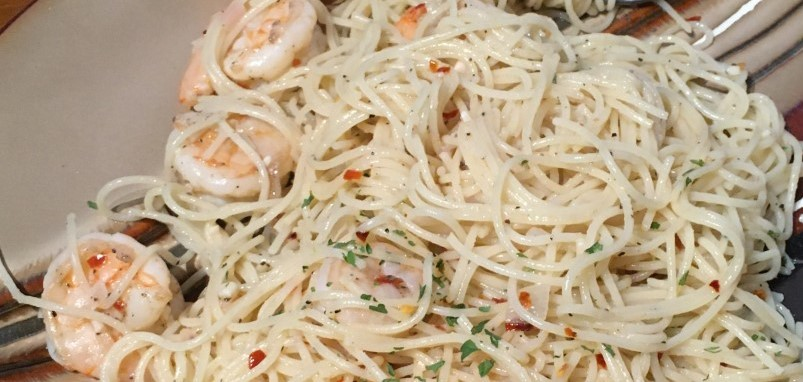
\includegraphics[scale=0.65]{Pasta/Shrimp Scampi/Shrimp Scampi.jpg}
%\end{center}

\end{document}